% Présentation de TeX et LaTeX
\small

\section{Présentation de \TeX\ et \LaTeX}

\subsection{Qu'est-ce que \TeX\ et \LaTeX?}

\begin{frame}[c,label=fr:commencement]{Au commencement (1978), il y eut \TeX\ldots}
	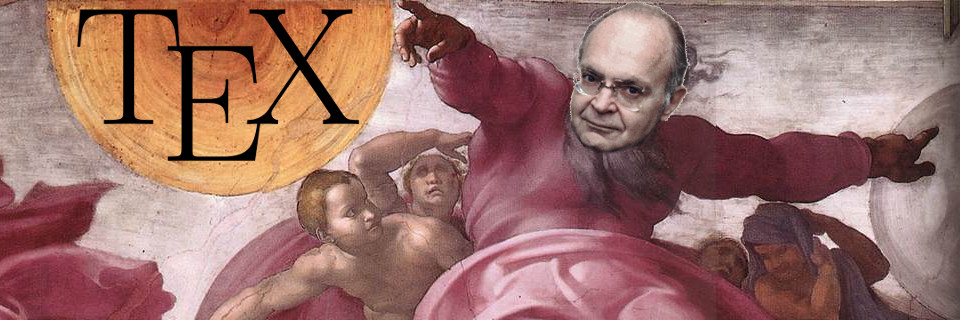
\includegraphics[width=\textwidth,keepaspectratio=true]{knuth-tex-commencement.jpg}
\end{frame}

\begin{frame}[c]{Qu'est-ce que \TeX?}

	\begin{itemize}
		\item Un système de mise en page (\emph{typesetting}) et de préparation de documents;
		\item «Le système le plus puissant pour produire des ouvrages scientifiques et
		techniques d'une grande qualité typographique»\footnote{Kopka \& Daly, p. 6};
		\item Un système mature, stable et complet, considéré comme exempt de bogues;
		\item Un ensemble de commandes très primitives parfaites pour la typographie et
		des fonctions de programmation;
		\item «\emph{typesetter-level program}».
	\end{itemize}

\end{frame}

\begin{frame}[c,label=fr:sixiemejour]{Au sixième jour (1983), il y eut \LaTeX\ldots}
	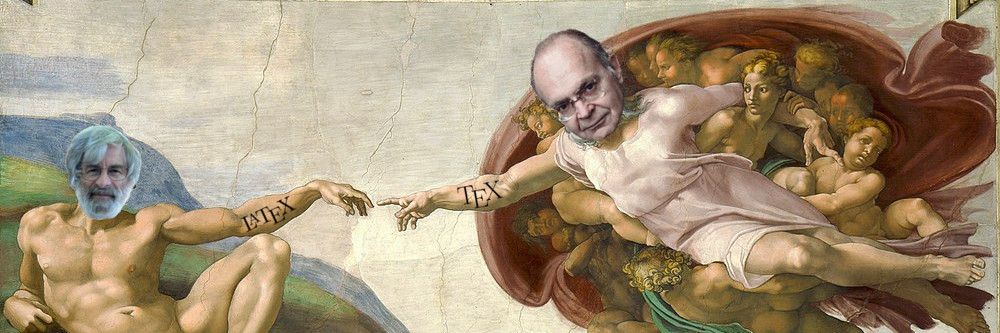
\includegraphics[width=\textwidth,keepaspectratio=true]{creation-of-latex.jpg}
\end{frame}

\begin{frame}{Qu'est-ce que \LaTeX?}
	\begin{itemize}
		\item Un ensemble de macro-commandes pour faciliter l'utilisation de \TeX.
		\item Ne requiert aucune connaissance préalable de la typographie en général et de \TeX\ en particulier.
		\item Langage de balisage (\emph{Markup Language}) typographique et logique pour indiquer la mise en forme du texte (pensez au HTML).
		\item Langage multiplateforme, identique d'un système d'exploitation à l'autre, et extensible par l'ajout de \emph{packages}.
		\item «\emph{author-level program}»
	\end{itemize}
\end{frame}

\subsection{Processus de création d'un document \LaTeX}

% Rédiger avec une nouvelle perspective
\begin{frame}[c]{Rédiger avec une nouvelle perspective}
	
	\begin{itemize}
		\item Vous rédigez votre document en texte brut et utilisez des commandes pour décrire
			\textbf{ce que votre texte représente} et \textbf{non pas ce à quoi il doit ressembler}.
		\item Vous vous concentrez sur votre \textbf{contenu}.
		\item Vous laissez \LaTeX\ faire son travail, c'est-à-dire s'occuper du \textbf{contenant}.
	\end{itemize}
	
\end{frame}

% Processus de création d'un document LaTeX
\begin{frame}[c]{Processus de création d'un document \LaTeX}
	\Huge
	\begin{minipage}[t]{0.25\linewidth}
		\centering
		\faFileTextO
	\end{minipage}
	\hfill\faArrowRight\hfill
	\begin{minipage}[t]{0.25\linewidth}
		\centering
		\faCogs
	\end{minipage}
	\hfill\faArrowRight\hfill
	\begin{minipage}[t]{0.25\linewidth}
		\centering
		\faFilePdfO
	\end{minipage}

	\begin{picture}(0,0)
		\footnotesize\thicklines\color{bleuFonceSecondaire}
		\onslide<2>\put(0,-10){\dashbox{1}(35,40)[b]{\parbox{.2\textwidth}{\centering\textbf{rédaction du texte et balisage avec éditeur de texte\smallskip}}}}
		\onslide<3>\put(54,-10){\dashbox{1}(35,40)[b]{\parbox{.2\textwidth}{\centering\textbf{compilation avec un moteur \TeX\ à partir de la ligne de commande\smallskip}}}}
		\onslide<4>\put(108,-10){\dashbox{1}(35,40)[b]{\parbox{.2\textwidth}{\centering\textbf{visualisation avec une visionneuse externe\smallskip}}}}
	\end{picture}
\end{frame}